\documentclass[11pt]{article}
\usepackage{amsmath}
\usepackage{amssymb}
\usepackage{graphicx}
\usepackage[margin=1in]{geometry}
% ---- exactly the lines from the worker's preamble.txt ----
\usepackage{tikz}
\usepackage{float}
% ---- end preamble.txt ----
\begin{document}
\section*{Problem zero (simulating a preceding fragment)}
Some preceding text so the fragment is not the first thing in the document.
\section*{Ex. 3.1 --- Loading the OS and one program without an MMU}

\paragraph{The constraint.}
With no MMU there is no translation step: the address the CPU puts on the bus is the
physical address. The program is linked to begin at 0 and to run over a contiguous
range, so physical address 0 and the bytes above it must belong to the application, and
the OS cannot have them.

\paragraph{The layout.}
Load the OS at the high end of RAM, growing downward from the physical top, and the
application at physical 0, growing upward: text, then data and bss, then the heap, with
the stack at the top of the user region growing down (Figure~\ref{p1:fig:memmap}). The
program owns the whole of $[0,F)$, where $F$ is the bottom of the OS, so both of the
CPU's assumptions hold with no translation and no relocation: the loader copies the
executable to address 0 byte for byte. Running a different program overwrites $[0,F)$;
the OS never moves.

\usetikzlibrary{decorations.pathreplacing}
\begin{figure}[H]
\centering
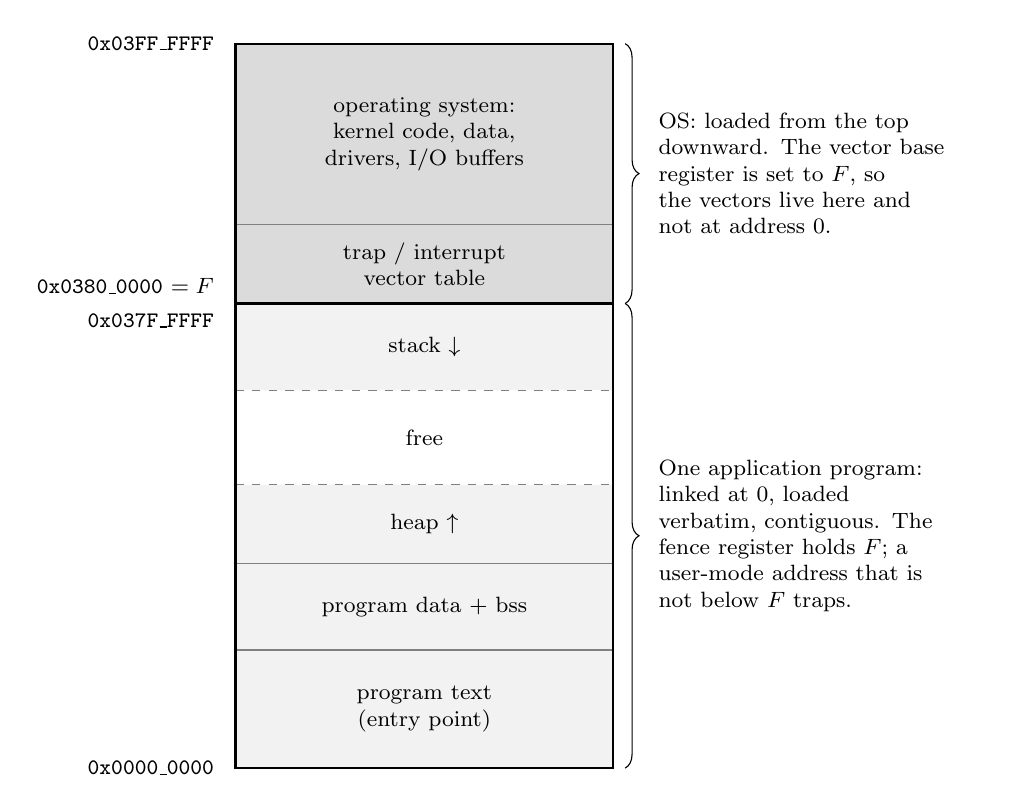
\begin{tikzpicture}[x=1cm,y=1cm,font=\footnotesize]
  \def\XL{0}\def\XR{4.8}
  % OS region (top)
  \fill[black!14] (\XL,5.9) rectangle (\XR,9.2);
  % program region bands
  \fill[black!5]  (\XL,0.0) rectangle (\XR,1.5);
  \fill[black!5]  (\XL,1.5) rectangle (\XR,2.6);
  \fill[black!5]  (\XL,2.6) rectangle (\XR,3.6);
  \fill[black!5]  (\XL,4.8) rectangle (\XR,5.9);
  % internal divisions
  \draw[gray] (\XL,1.5) -- (\XR,1.5);
  \draw[gray] (\XL,2.6) -- (\XR,2.6);
  \draw[gray,dashed] (\XL,3.6) -- (\XR,3.6);
  \draw[gray,dashed] (\XL,4.8) -- (\XR,4.8);
  \draw[gray] (\XL,6.9) -- (\XR,6.9);
  % outline and the fence boundary
  \draw[thick] (\XL,0) rectangle (\XR,9.2);
  \draw[very thick] (\XL,5.9) -- (\XR,5.9);
  % region labels
  \node[align=center] at (2.4,8.05) {operating system:\\ kernel code, data,\\ drivers, I/O buffers};
  \node[align=center] at (2.4,6.40) {trap / interrupt\\ vector table};
  \node[align=center] at (2.4,5.35) {stack $\downarrow$};
  \node[align=center] at (2.4,4.20) {free};
  \node[align=center] at (2.4,3.10) {heap $\uparrow$};
  \node[align=center] at (2.4,2.05) {program data + bss};
  \node[align=center] at (2.4,0.75) {program text\\ (entry point)};
  % addresses on the left
  \node[anchor=east] at (-0.15,9.20) {\texttt{0x03FF\_FFFF}};
  \node[anchor=east] at (-0.15,6.12) {\texttt{0x0380\_0000} $= F$};
  \node[anchor=east] at (-0.15,5.68) {\texttt{0x037F\_FFFF}};
  \node[anchor=east] at (-0.15,0.00) {\texttt{0x0000\_0000}};
  % spans on the right
  \draw[decorate,decoration={brace,amplitude=5pt}] (\XR+0.15,9.2) -- (\XR+0.15,5.9);
  \draw[decorate,decoration={brace,amplitude=5pt}] (\XR+0.15,5.9) -- (\XR+0.15,0.0);
  \node[anchor=west,align=left,text width=4.1cm] at (\XR+0.45,7.55)
       {OS: loaded from the top\\ downward. The vector base\\ register is set to $F$, so\\ the vectors live here and\\ not at address 0.};
  \node[anchor=west,align=left,text width=4.1cm] at (\XR+0.45,2.95)
       {One application program:\\ linked at 0, loaded\\ verbatim, contiguous. The\\ fence register holds $F$; a\\ user-mode address that is\\ not below $F$ traps.};
\end{tikzpicture}
\caption{Memory map for a single-program system with no MMU. Physical memory is
64\,MiB and the OS occupies the top 8\,MiB. Addresses increase upward.}
\label{p1:fig:memmap}
\end{figure}

\paragraph{Address 0 is not usually free.}
Most CPUs fetch trap and interrupt vectors from fixed low addresses: the 68000's table
at \texttt{0x000}--\texttt{0x3FF}, x86 real mode's IVT at
\texttt{0x00000}--\texttt{0x003FF}, ARM's vectors at 0. That collides with the layout,
so I require a CPU with a vector base register (68010 VBR, ARM VBAR, RISC-V
\texttt{mtvec}) and set it to $F$. Such a register is consulted only when an exception
is dispatched and leaves ordinary loads and stores untouched, so it is not an MMU. On a
CPU that hard-wires its vectors at 0 the assumption cannot be met: the vectors keep the
low addresses and the program has to be relocated when it is loaded. Only the reset
vector cannot be moved in principle, and it is served from boot ROM.

\paragraph{The boundary.}
No MMU also means no permission check per access, so nothing above stops the application
from storing into the OS. I therefore allow one fence (limit) register holding $F$: in
user mode the CPU traps any address that is not below $F$. A comparison adds nothing to
the address, so this is still not translation; a \emph{base} register, added to every
address, is where an MMU begins.

\section*{Problem two (simulating a following fragment)}
Some following text.
\end{document}
